

\documentclass{beamer}

% Theme choice:
\usetheme{CambridgeUS}

% Title page details: 

\usepackage{polynom}
\usepackage{amssymb}
\usepackage{amsmath}

\usepackage{bm}
\usepackage[misc]{ifsym}

\usepackage{enumitem}
\usepackage{mathtools}
\usepackage[applemac]{inputenc}
\usepackage{tikz}

\usepackage{parskip}

\DeclareMathOperator*{\Res}{Res}
\DeclareMathOperator*{\equals}{=}
\DeclareMathOperator*{\pipe}{|}

\hyphenation{op-tical net-works semi-conduc-tor}
\def\inputGnumericTable{}  
\graphicspath{{./images/}}


\begin{document}
\newcommand{\bfr}[2]{\section{#1} \begin{frame}{#1} #2 \end{frame}}

	\title{Assignment 12}
		\author{ Abhay Shankar K: CS21BTECH11001}
\date{}
	\begin{frame}
    		\titlepage
	\end{frame}

	\begin{frame}{Outline}
    		\tableofcontents
	\end{frame}

	\providecommand{\brak}[1]{\ensuremath{\left(#1\right)}}
	\providecommand{\mn}[2]{\ensuremath{min\brak{#1, #2}}}
	\providecommand{\mx}[2]{\ensuremath{max\brak{#1, #2}}}
	\providecommand{\rpr}[2]{\ensuremath{P_{#1}\left(#2\right)}} %random variable notation
	\providecommand{\spr}[1]{\ensuremath{P\left(#1\right)}} %simple notation
	\newcommand{\abs}[1]{\left| #1 \right|}
    \newcommand{\e}[1]{\ensuremath{e^{#1}}}

    \providecommand{\myroman}{\brak{\textbf{\roman*}}}
	
	\providecommand{\pdf}[2]{\ensuremath{p_{#2}\left(#1\right)}}
	\providecommand{\cdf}[2]{\ensuremath{P_{#2}\left(#1\right)}}
    \providecommand{\inv}[1]{\ensuremath{\frac{1}{#1}}}
    
	
	\bfr{Question}{
		Given a Wiener process $w\brak{t}$ with parameter $\alpha$, we form the processes
        \begin{enumerate}[label = \textbf{\brak{\roman*}}]
            \item $x\brak{t} = w\brak{t^2}$
            \item $y\brak{t} = w^2\brak{t}$
            \item $z\brak{t} = \abs{w\brak{t}}$
        \end{enumerate}

        Show that $x\brak{t}$ is normal with zero mean. Furthermore, if $t_1 < t_2$,
        \begin{enumerate}[label = \textbf{\brak{\arabic*}}]
            \item $R_x\brak{t_1, t_2} = \alpha t_1^2$
            \item $R_y\brak{t_1, t_2} = \alpha^2 t_1 \brak{2t_1 + t_2}$
            \item $R_z\brak{t_1, t_2} = \frac{2 \alpha}{\pi} \sqrt{t_1 t_2} \brak{\cos{\theta} + \pi \sin{\theta}}$
        \end{enumerate} 
        where $\theta = \sin^{-1}(\sqrt{\frac{t_1}{t_2}})$
	}

    \bfr{Finding $x(t), y(t), \& z(t)$}{
        \begin{align}
            \pdf{t}{w} &= \inv{\sqrt{2 \pi \alpha t}} \e{-\frac{x^2}{2 \alpha t}} \nonumber \\
            \implies \pdf{t}{x} &= \inv{\sqrt{2 \pi \alpha }t} \e{-\frac{x^2}{2 \alpha t^2}} \\
            \text{Putting } \sigma &= t \sqrt{\alpha}, \nonumber \\
            \pdf{t}{x} &= \inv{\sigma \sqrt{2 \pi}} \e{-\frac{x^2}{2\sigma^2}} \nonumber
        \end{align}
        which is clearly Gaussian with variance $\alpha t^2$. Also,
        \begin{align}
            E[x(t)] &= 0 \nonumber \\
            E[x^2(t)] &= Var[x(t)] + E^2[x(t)] \nonumber \\
            &= \alpha t^2
        \end{align}
    }
    \bfr{}{
        Due to the standard formula for the distribution of the square of a given RV, 
        \begin{align}
            \pdf{t, x}{y} &= \inv{\sqrt{x}} \pdf{t, \sqrt{x}}{w} \nonumber \\
            &= \inv{\sqrt{2 \pi \alpha t x}} \e{-\frac{x}{2 \alpha t}} \\
            \nonumber \\
            \therefore E[y(t)] &= \int_0^\infty x \inv{\sqrt{2 \pi \alpha t x}} \e{-\frac{x}{2 \alpha t}} dx \nonumber \\
            &= \alpha t \\
            E[y^2(t)] &= \int_0^\infty x^2 \inv{\sqrt{2 \pi \alpha t x}} \e{-\frac{x}{2 \alpha t}} dx \nonumber \\
            &= 3(\alpha t^2)
        \end{align}
    }

    \bfr{}{
        We know the half normal distribution, by definition,
        \begin{align}
            \pdf{x, t}{z = \abs{w}} &= 2 u(x) \inv{\sqrt{2 \pi \alpha t}} \e{-\frac{x^2}{2 \alpha t}} \\
            \therefore E[z(t)] &= 2 \int_0^\infty x \inv{\sqrt{2 \pi \alpha t x}} \e{-\frac{x^2}{2 \alpha t}} dx \nonumber \\
            &= \sqrt{\frac{2 \alpha t}{\pi}} \\
            E[z^2(t)] &= \int_0^\infty x^2 \inv{\sqrt{2 \pi \alpha t x}} \e{-\frac{x^2}{2 \alpha t}} dx \nonumber \\
            &= \alpha t 
        \end{align}
    }
	
    \bfr{Finding Autocorrelation}{
        \begin{align}
            R_x(t_1, t_2) &= E[x(t_1)x(t_2)] \nonumber\\
            &= E[x(t_1)]E[x(t_2) - x(t_1)] + E[x^2(t_1)] \nonumber\\
            &= E[x^2(t_1)] \nonumber \\
            &= \alpha t_1^2 \label{rx} \\
    \nonumber \\
            R_y(t_1, t_2) &= E[y(t_1)y(t_2)] \nonumber \\
                &= E[y(t_1)]E[y(t_2) - y(t_1)] + E[y^2(t_1)] \nonumber \\
                &= \alpha t_1 (\alpha t_2 - \alpha t_1) + 3 (\alpha t_1)^2 \nonumber \\
                &= \alpha^2 t_1(2t_1 + t_2) \label{ry}
        \end{align}
    }
    \bfr{}{
        \begin{align}
            R_z(t_1, t_2) &= E[z(t_1)z(t_2)] \nonumber \\
            &= E[z(t_1)]E[z(t_2) - z(t_1)] + E[z^2(t_1)] \nonumber \\
            &= \frac{2 \alpha}{\pi} \sqrt{t_1 t_2}(\sqrt{1 - \frac{t_1}{t_2}} + \pi \sqrt{\frac{t_1}{t_2}}) \nonumber \\
            &= \frac{2 \alpha}{\pi} \sqrt{t_1 t_2} (\cos{\theta} + \pi \sin{\theta})
        \end{align}
    }
	

	\bfr{Graph}{
		\begin{figure}[h!]
			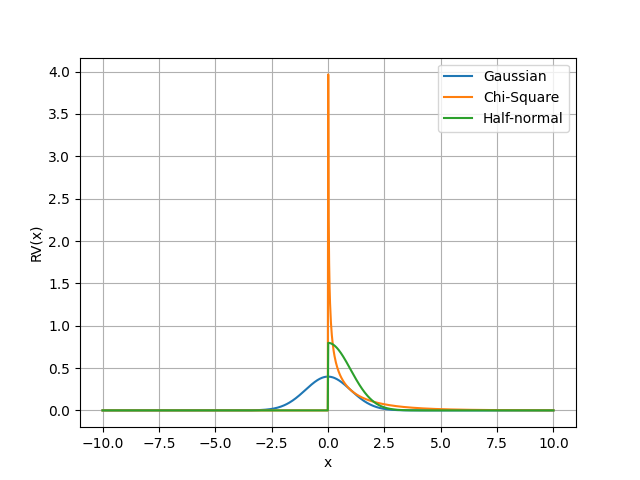
\includegraphics[scale = 0.6]{assig12_3g.png}
		\end{figure}
	}
	
								
\end{document}
	
	

	
	
	
	